\documentclass[a4paper,11pt]{article}

\usepackage{amsmath}
\usepackage{amssymb}

% for proofs  environment
\usepackage{amsthm}

\usepackage[backend=bibtex]{biblatex}
\bibliography{reading5aThink}

% for probability trees
\usepackage{tikz}
\usetikzlibrary{trees}

% for plots
\usepackage{pgfplots}

%for strikethrough text
\usepackage{soul}

%for R source code listing
\usepackage{listings}

%for block quotes
\usepackage{csquotes}

% For not indenting the first line of paragraphs:
\setlength{\parindent}{0pt}
% define the title
\author{John Hancock}
\title{MIT Introduction to Statistics 18.05 Problem Set 2 }
\begin{document}
% generates the title
\maketitle
% insert the table of contents
\tableofcontents
\section{References and License}
We are answering questions in the material from MIT OpenCourseWare
course 18.05, Introduction to Probability and Statistics.

Please see the references section for detailed citation information.

The material for the course is licensed under the terms at
\url{http://ocw.mit.edu/terms}.

We are answering the questions that Orloff and Bloom ask in
\cite{reading5a}.

We use documentation in \cite{basicPlot}, \cite{plotGallery} to
write \LaTeX source code for this document.

\section{Higest variance for Bernoulli}
In this section we answer the think question, ``For what value of p does
Bernoulli(p) have the highest variance? Try to answer this by plotting the PMF
for various p.''

We plot the PMF for values of $p$: $0.0$, $0.1$, $0.3$, $0.5$, and $0.7$:

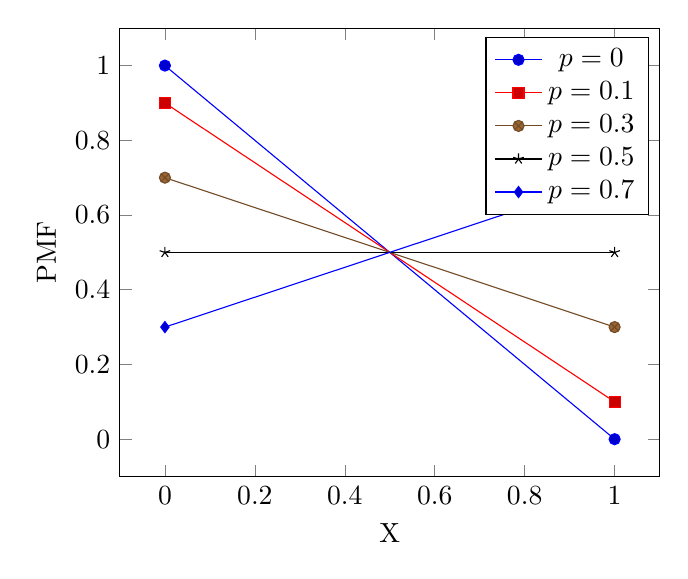
\begin{tikzpicture}
\begin{axis}[
	xlabel={X},
	ylabel={PMF}
]
\addplot coordinates {
	(0,1)    (1,0)
};

\addplot coordinates{
	(0,0.9)    (1,0.1)
};

\addplot coordinates{
	(0,0.7)    (1,0.3)
};

\addplot coordinates{
	(0,0.5)    (1,0.5)
};

\addplot coordinates{
	(0,0.3)    (1,0.7)
};
\legend{$p=0$,$p=0.1$,$p=0.3$,$p=0.5$,$p=0.7$}
\end{axis}
\end{tikzpicture}

We see that the largest spread in values of the PMF is where $p$ is close to
0 or close to 1.

\printbibliography{}
\end{document}
